\documentclass[%
12pt, %
final, % 
oneside, % 
onecolumn, %  
centertags]{article} % относится к классу article и размер шрифта 12 пунктовб, {article: статья, report: отчеты и диссертации, book: книга, letter: письмо}

% \usepackage{fontspec}
 
% \setmainfont{Times New Roman}

% \documentclass[a4paper, 12pt]{report}

\topmargin= -30pt % насколько сверху будет страница
\textheight= 650pt


\usepackage[utf8]{inputenc} % задает кодировку, utf-8 кодировка, включающая в себя знаки почти всех языков мира
\usepackage[english]{babel} % подключает необходимые языки, основным языком является английский

\selectlanguage{english} % настройки будут на английском, но писать будет на русском

\usepackage{euscript}
\usepackage{supertabular}

\renewcommand{\baselinestretch}{1.0} 

\usepackage[colorlinks=true,linkcolor=blue,unicode=true,urlcolor = blue]{hyperref} %hypered
\usepackage[pdftex]{graphicx} % для графики

\usepackage{amsthm, amssymb, amsmath, amsfonts} % математический пакет, математические шрифты
\usepackage{textcomp}
\usepackage[noend]{algorithmic}
\usepackage[ruled]{algorithm}
\usepackage{lipsum}
\usepackage{indentfirst}
\usepackage{babel}
\usepackage{pgfplots}
\usepackage{setspace}
\usepackage{xcolor}
\usepackage{hyperref}
\usepackage{subfigure}

\setcounter{secnumdepth}{5}
\setcounter{tocdepth}{5}
\newcommand\simpleparagraph[1]{%
  \stepcounter{paragraph}\paragraph*{\theparagraph\quad{}#1}}
\usepackage{listings}
% \usepackage{xcolor}
%\usepackage{minted}

\lstset { %
     language=C++,
     backgroundcolor=\color{black!5}, % set backgroundcolor
     basicstyle=\footnotesize,% basic font setting
}


\linespread{1.0} 
\setlength{\parindent}{2.4em}
\setlength{\parskip}{0.1em}

\pgfplotsset{compat=1.9}
\pgfplotsset{model/.style = {blue, samples = 100}} 
\pgfplotsset{experiment/.style = {red}}

\theoremstyle{plain}
\binoppenalty=10000

\newtheorem{theorem}{Theorem}[section] % theorem

\theoremstyle{definition}
% \newtheorem{definition}{Определение}[subsection]
\newtheorem{definition}{Definition}[subsection]

\theoremstyle{remark}
% \newtheorem{remark}{Замечание}[section]

% \newtheorem{corollary}{Следствие}

% \newtheorem{proposition}{Proposition}

% \newtheorem{example}{Пример}

% \newtheorem{lemma}{Лемма}[section]

\renewcommand*{\proofname}{Proof}

\graphicspath{ {./images/} }


% \usepackage{amsmath,amsfonts,amssymb, setspace}  % Разнообразные математические команды и значки
% \usepackage{indentfirst}     % Отступ в первом абзаце

% \pagestyle{empty}
\usepackage[left=2.5cm, right=1.5cm, top=2.5cm, bottom=2.5cm]{geometry}
\usepackage[medium]{titlesec}
\usepackage{graphicx}
% \graphicspath{ {./images/} }

\begin{document}

	\begin{titlepage} 
		\begin{center}
		\textbf{}\\[2.0cm]
		\LARGE FEDERAL STATE AUTONOMOUS EDUCATIONAL INSTITUTION OF HIGHER EDUCATION \\[0.5cm]
		\Large ITMO UNIVERSITY \\[3cm]
		\LARGE Report\\
		\Large MPI. Assignments $16-17$ \\
		\Large Parallel algorithms for the analysis and synthesis of data \\[4cm]


		\begin{flushright}
		Performed by\\
		Aleksandr Shirokov\\
		J4133c\\
		Accepted by\\
		Petr Andriushchenko

		Deadline: 24.12.21
		\end{flushright}

		\vfill 

		{\Large {St. Petersburg}} \par
		{\Large {2021}}
		\end{center} 
	\end{titlepage}

\tableofcontents
\newpage


\section{Assignments}

\subsection{Assignment 16. MPI. Operations with communicators. Renumbering processes.}

\subsubsection{Formulation of the problem}

In the \textsc{MPI\_Comm\_split} function (\textsc{Assignment16.c}), replace the color parameter with (rank\% 2), (rank\% 3), 
look at how many groups the processes are split into, depending on the specified attribute of division into 
groups.

int \textbf{MPI\_Comm\_split} (
\begin{itemize}
	\item IN MPI\_Comm \textbf{comm} - parent communicator
	\item IN int \textbf{color} - a sign of division into groups
	\item IN int \textbf{key} - parameter defining numbering in new groups
	\item OUT MPI\_Comm *\textbf{newcomm} - new communicator
\end{itemize}
)

The function splits the group associated with the parent communicator into non-overlapping subgroups, one 
for each value of the color subgroup attribute. \textbf{Color} must be non-negative. Each subgroup contains 
processes with the same color value. The \textbf{key} parameter controls the ordering within the new groups: a 
lower \textbf{key} value corresponds to a lower process ID value. If the \textbf{key} parameter is equal for multiple 
processes, the ordering is performed according to the order in the parent group

\subsubsection{Example of launch parameters and output. Detailed description of solution}

Code for \textbf{assignment 16} is \href{https:\//github.com/aptmess/parallel_algorithms/blob/master/HT/hw_mpi/Assignment16.c}{here}.

Compilation example: \textsc{mpic++ -o ./cpf/16.o Assignment16.c}

Launch example: 

\begin{enumerate}
	\item \textsc{mpirun --oversubscribe -np 4 ./cpf/16.o 2}
	\item \textsc{mpirun --oversubscribe -np 4 ./cpf/16.o 3}
\end{enumerate}

\begin{center}
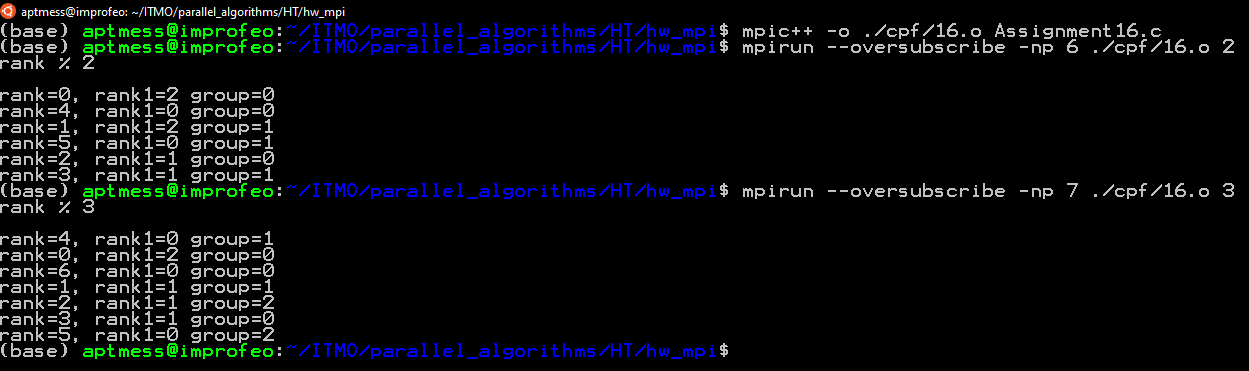
\includegraphics[scale=0.55]{16.png}
\end{center}

Let's move to the the code and explain how it works.

\begin{center}
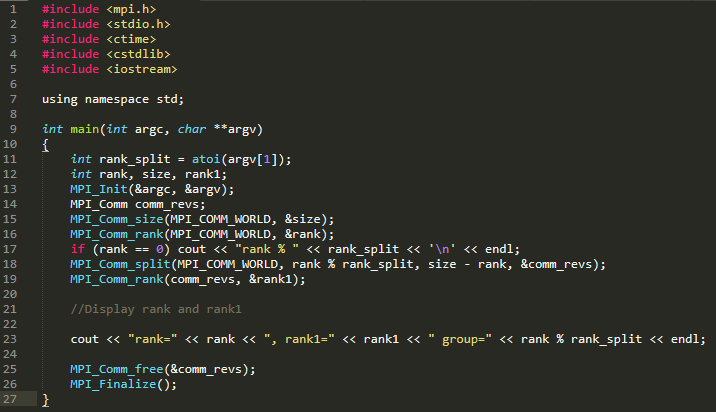
\includegraphics[scale=0.9]{16.code.png}

Assignment16 code
\end{center}

This program works clearly - all processes are splitted into groups based on some condition such as $\operatorname{color}=\operatorname{rank} \% 2$ or $\operatorname{color}=\operatorname{rank} \% 3$ and the new rank in group is calculated as $\operatorname{size} - rank$ as a \textsc{rank1} variable with process rank in new group. For example for second run example, with initial $7$ processes they are splitted on three groups: $0: \{0, 3, 6\}, 1: \{1, 4\}, 2: \{3, 5\}$ and new ranks are $0: \{2, 1, 0\}, 1: \{1, 0\}, 2: \{1, 0\}$ as on a screen higher. The program is tested and works correctly.

\newpage
\subsection{Assignment 17. MPI. Data packing. Sending packed data.}

\subsubsection{Formulation of the problem}

Understand the new functions in \textsc{Assignment17.c} and explain program execution.

Display the values of the process number and arrays $a[i]$, $b[i]$, before packing and 
distribution, and after. See how broadcasting works.

\subsubsection{Example of launch parameters and output. Detailed description of solution}

Code for \textbf{assignment 17} is \href{https:\//github.com/aptmess/parallel_algorithms/blob/master/HT/hw_mpi/Assignment17.c}{here}.

Compilation example: \textsc{mpic++ -o ./cpf/17.o Assignment17.c}

Launch example: \textsc{mpirun --oversubscribe -np 4 ./cpf/17.o}

\begin{center}
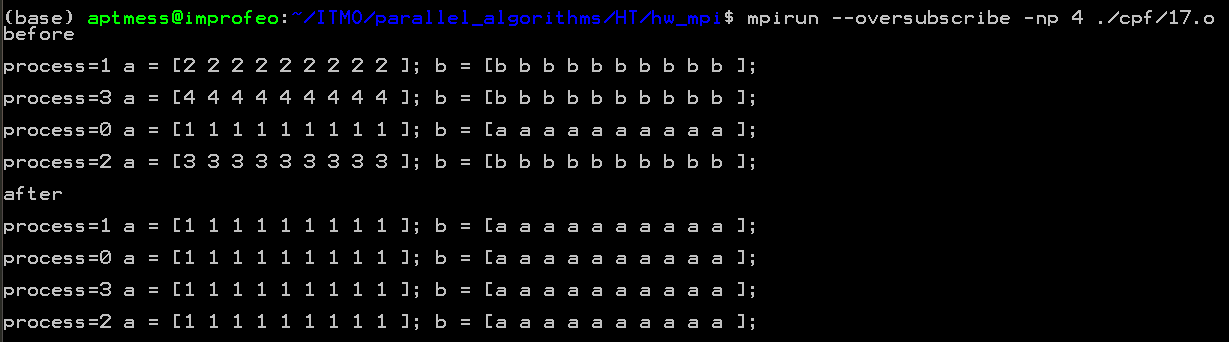
\includegraphics[scale=0.55]{17.png}
\end{center}

Let's move to the the code and explain how it works.

\begin{center}
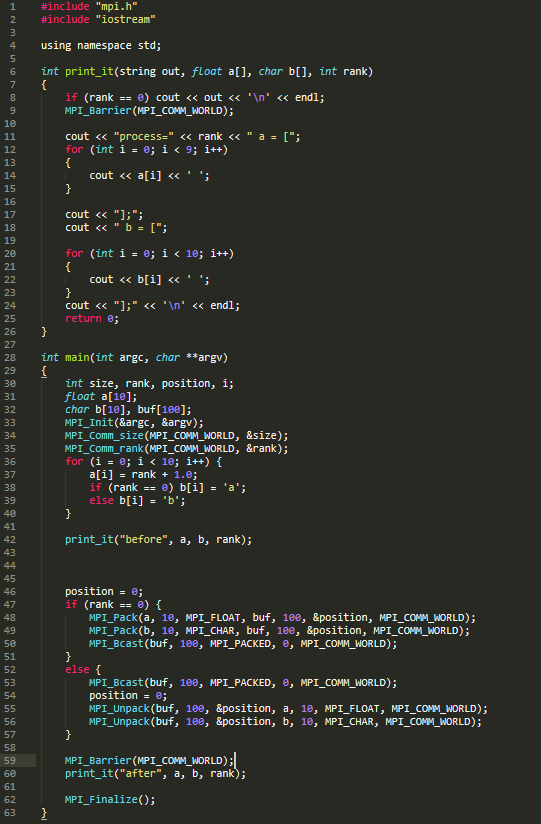
\includegraphics[scale=0.9]{17.code.png}

Assignment17 code
\end{center}

Theare are three new functions in the code:
\begin{itemize}
	\item int MPI\_Pack that packs a datatype into contiguous memory(
	\begin{itemize}
		\item const void *inbuf - input buffer start (choice)
		\item int incount - number of input data items (non-negative integer)
		\item MPI\_Datatype datatype - datatype of each input data item (handle)
		\item OUT - void *outbuf - output buffer start (choice)
		\item int outsize - output buffer size, in bytes (non-negative integer)
		\item IN/OUT int *position - current position in buffer, in bytes (integer)
		\item MPI\_Comm comm - communicator for packed message (handle)
	\end{itemize}
	\item int MPI\_Unpack that unpack a buffer according to a datatype into contiguous memory(
	\begin{itemize}
		\item const void *inbuf - input buffer start (choice)
		\item int insize - size of input buffer, in bytes (integer)
		\item IN/OUT int *position - current position in buffer, in bytes (integer)
		\item OUT - void *outbuf - output buffer start (choice)
		\item int outcount - number of items to be unpacked (integer)
		\item MPI\_Datatype datatype - datatype of each output data item (handle)
		\item MPI\_Comm comm - communicator for packed message (handle)
	\end{itemize}
	\item \textsc{MPI\_Bcast} broadcasts a message from the main process ($rank=0$) to all other processes of the communicator
\end{itemize}

Due to this our function works like this - there are initliazation of two arrays, first array $a$ is filled by formula 'current rank + 1' and the other $b$ contains char 'a' if it is root process and 'b' if not. After that i am printing array and if it is root process array $a$ and $b$ due to function \textsc{MPI\_Pack} are packing into one contiguous memory and after packing thia arrays are cast to other processes using \textsc{MPI\_Bcast}. In others processes using \textsc{MPI\_Unpack} function we are unpacking a buffer from process $0$ accodring to datatypeto contigious memory and as we expected the messages in non root processes in arrays $a$ and $b$ are overwritten by root values in this arrays. The proram is explained and works correctly.
\subsection{Appendix}
 
The link to the sourse code which is placed on my \href{https://github.com/aptmess/parallel_algorithms}{github}.


\end{document}